\newpage
\section{پرسش های متداول\label{faq}}

در این بخش برخی از سوالات متداول که کاربران میپرسند به مرور زمان اضافه میشود.

\begin{question}{مشخصات فنداسیون یا پانچ برای من نمایش داده نمیشود.}
\true 
اگر با کلیک روی فنداسیون یا هر یک از ستونها در محیط سه بعدی یا قسمت بالایی جدول
\lr{Combo View}
مشخصات فنداسیون یا پانچ ها قابل مشاهده نیستند، در قسمت پایین جدول مطمئن شوید که تب 
\lr{Data}
فعال باشد، مطابق شکل
\ref{fig:dataview}.
\end{question}

\begin{figure}[H]
    \centering
    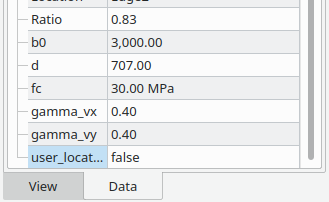
\includegraphics{figures/dataview}
    \caption{تنظیم نمایش مشخصات با انتخاب تب \lr{Data}}
    \label{fig:dataview}
\end{figure}


\begin{question}{چطور هر بار که نرم افزار را باز میکنم به طور خودکار 
    \lr{Civil}
    لود شود؟}
\true 
برای این کار باید از منوی
$Edit \rightarrow Preferences$
پنجره تنظیمات نرم افزار را باز کنید. مطابق شکل
\ref{fig:autoload}
، در تب
\lr{General}
قسمت 
\lr{Start up}
ورک بنچ 
\lr{Civil}
را انتخاب کنید و سپس کلید تایید را بزنید. از این پس بعد از اجرای نرم افزار به طور خودکار ورک بنچ
\lr{Civil}
لود میشود.
\end{question}


\begin{figure}[H]
    \centering
    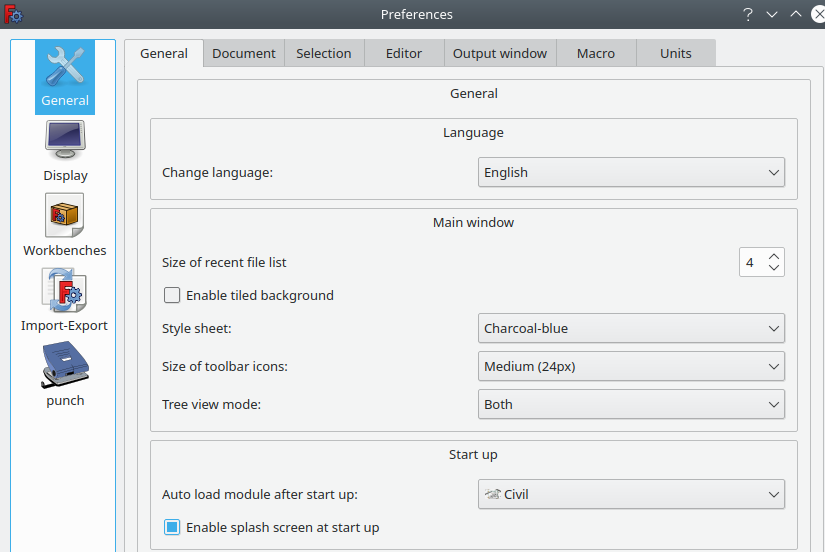
\includegraphics[width=.7\linewidth]{figures/autoload}
    \caption{تنظیم لود شدن خودکار ورک بنچ \lr{Civil} بعد از هر اجرا}
    \label{fig:autoload}
\end{figure}